\chapter{Stato dell'arte}
\label{cha:statoArte}

\section{Reverse Proxy}
\subsection{Cos'é}
Un reverse proxy é un dispositivo che fa da intermediario tra i server presenti sotto una rete locale e la rete esterna. Le comunicazioni in uscita dai server passano quindi dal reverse proxy e poi vanno verso gli utenti, e uguale quelle in ingresso, entrano nella rete locale attraverso il reverse proxy e poi vengono indirizzate ai server desiderati.
\begin{figure}[h!]
  \centering
  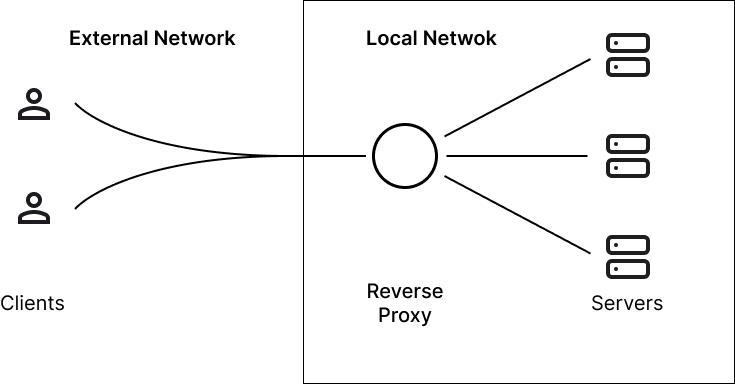
\includegraphics[width=.6\textwidth]{images/schema.png}
\end{figure}

\subsection{Perché viene utilizzato}
L'utilizzo di una struttura che si pone in mezzo alle comunicazioni garantisce molti vantaggi visto che ha accesso a tutte le comunicazioni entranti. Il reverse proxy puó quindi analizzare le connessioni ed effettuare delle operazioni con queste ultime come ad esempio controlli per motivi di sicurezza, chaching e load balancing. Inoltre in questo modo si puó accedere a piú servizi tramite lo stesso nodo di ingresso.

\subsection{Funzionalitá}
Analizziamo adesso le funzionalitá che un reverse proxy puó offrire.

\subsubsection{Sicurezza}
Sicuramente le funzionalitá piú importanti sono quelle relative alla sicurezza. Un reverse proxy infatti ne implementa molte evitando la necessitá di implementare sistemi di sicurezza per ogni servizio che andiamo ad inserire nella rete locale.
\begin{enumerate}
  \item \textbf{TLS}: Ogni comunicazioni in ingresso e in uscita puó essere criptata tramite il protocollo TLS.
  \item \textbf{controllo attacchi DoS/DDoS}: Controllando tutte le comunicazioni e i relativi ip sorgente, si possono applicare filtri e controlli per evitare un eccesso di richieste in entrata che possono rallentare le funzionalitá dei server.
  \item \textbf{supporto protocolli piú recenti}: Il reverse proxy puó supportare protocolli piú recenti rispetto ai server cosí la connessione interna tra servere e reverse proxy puó essere effettuata nel protocollo piú recente supportata dal server, ma poi quella all'esterno puó essere elevata ad un protocollo piú recente e quindi con maggiore sicurezza.

\end{enumerate}

\subsubsection{Prestazioni}
\begin{enumerate}
  \item \textbf{TLS}: Criptare la comunicazione nel nodo del reverse proxy e lasciando la comunicazione interna in chiaro allegerisce molto il carico di lavoro ai server.
  \item \textbf{Cache}: Implementando un sistema di caching, richieste ricorrenti alle stesse risorse possono essere soddisfatte direttamente dal reverse proxy, senza inoltrare la richiesta al server.
  \item \textbf{Compressione}: Comprimere le risposte cosí da occupare meno banda e non influire sulle prestazioni dei server in quanto il processo di compressione e decompressione delle richieste é effettuato dal reverse proxy.
\end{enumerate}

\subsubsection{Load Balancer}
Se si hanno piú server (macchine) che rispondono alle stesse richieste, si possono indirizzare le richieste in modo che carico di lavoro sia distribuito equamente tra i vari server. In base all'algoritmo implementato il processo di load balancing puó essere fatto in modo accurato oppure piú grezzo. L'algoritmo scelto dipende molto dal caso d'uso.

\section{SSL/TLS}
